% !TeX document-id = {3b8d65d3-a02c-4f16-abb9-6a325ca708dd}
% !TeX TXS-program:compile = txs:///latex/[--shell-escape]|txs:///dvips|txs:///ps2pdf
\documentclass[10pt,a4paper]{article}
\usepackage[spanish]{babel}
\usepackage[utf8]{inputenc}
\usepackage{fancyhdr} %header
\usepackage{amsmath}
\usepackage{amsfonts}
\usepackage{amssymb}
\usepackage{minted} % coloreado de codigo
\usepackage{listings}
\usepackage{caption}
\usepackage{subcaption} % side by side figures
% grafico
% grafo
\usepackage{float} % para forzar las imagenes
\usepackage[usenames,dvipsnames, pdf]{pstricks}
\usepackage{epsfig}
\usepackage{pst-grad} % For gradients
\usepackage{pst-plot} % For axes
\usepackage[space]{grffile} % For spaces in paths
\usepackage{etoolbox} % For spaces in paths
\makeatletter % For spaces in paths
\patchcmd\Gread@eps{\@inputcheck#1 }{\@inputcheck"#1"\relax}{}{}
\makeatother
%
\author{Iñigo Biedma Ramos}
\title{Entrega Práctica Genéticos TSP}
\date{}
\renewcommand{\theenumi}{\alph{enumi}}
\pagestyle{fancy}
\fancyhf{}
\lhead{Entrega Práctica Genéticos TSP - Computación}
\rhead{Iñigo Biedma Ramos}
\begin{document}
\maketitle
\section{el modelo}
\subsection{Cromosomas}
A la hora de representar el problema del TSP existen dos formas básicas de representarlo: Representar la posicion de las ciudades, o representar la distancia entre ellas. Lo más habitual es representar las distancias, y de hecho eso 
\begin{figure}[H]
	\centering
	%\usepackage[usenames,dvipsnames]{pstricks}
%\usepackage{epsfig}
%\usepackage{pst-grad} % For gradients
%\usepackage{pst-plot} % For axes
%\usepackage[space]{grffile} % For spaces in paths
%\usepackage{etoolbox} % For spaces in paths
%\makeatletter % For spaces in paths
%\patchcmd\Gread@eps{\@inputcheck#1 }{\@inputcheck"#1"\relax}{}{}
%\makeatother
% % User Packages:
% 
% 
\psscalebox{0.4 0.4} % Change this value to rescale the drawing.
{
\begin{pspicture}(0,-5.6)(20.0,5.6)
\psellipse[linecolor=black, linewidth=0.04, dimen=outer](4.0,0.8)(0.4,0.4)
\pscircle[linecolor=black, linewidth=0.04, dimen=outer](4.0,4.8){0.4}
\pscircle[linecolor=black, linewidth=0.04, dimen=outer](6.4,3.6){0.4}
\pscircle[linecolor=black, linewidth=0.04, dimen=outer](1.6,3.6){0.4}
\psline[linecolor=black, linewidth=0.04](4.4,0.8)(6.4,3.2)
\psline[linecolor=black, linewidth=0.04](6.4,4.0)(4.4,4.8)
\psline[linecolor=black, linewidth=0.04](3.6,4.8)(1.6,4.0)
\psline[linecolor=black, linewidth=0.04](1.6,3.2)(3.6,0.8)
\psdots[linecolor=black, dotsize=0.4](6.4,3.6)
\psellipse[linecolor=black, linewidth=0.04, dimen=outer](10.4,0.8)(0.4,0.4)
\pscircle[linecolor=black, linewidth=0.04, dimen=outer](10.4,4.8){0.4}
\pscircle[linecolor=black, linewidth=0.04, dimen=outer](12.8,3.6){0.4}
\pscircle[linecolor=black, linewidth=0.04, dimen=outer](8.0,3.6){0.4}
\psdots[linecolor=black, dotsize=0.4](12.8,3.6)
\psline[linecolor=black, linewidth=0.04](12.8,3.2)(10.8,0.8)
\psline[linecolor=black, linewidth=0.04](10.4,1.2)(10.4,4.4)(10.4,4.4)
\psline[linecolor=black, linewidth=0.04](10.0,4.8)(8.0,4.0)(8.0,4.0)
\psline[linecolor=black, linewidth=0.04](12.8,4.0)(8.0,3.2)
\psellipse[linecolor=black, linewidth=0.04, dimen=outer](4.0,-4.8)(0.4,0.4)
\pscircle[linecolor=black, linewidth=0.04, dimen=outer](4.0,-0.8){0.4}
\pscircle[linecolor=black, linewidth=0.04, dimen=outer](6.4,-2.0){0.4}
\pscircle[linecolor=black, linewidth=0.04, dimen=outer](1.6,-2.0){0.4}
\psdots[linecolor=black, dotsize=0.4](6.4,-2.0)
\psellipse[linecolor=black, linewidth=0.04, dimen=outer](16.8,0.8)(0.4,0.4)
\pscircle[linecolor=black, linewidth=0.04, dimen=outer](16.8,4.8){0.4}
\pscircle[linecolor=black, linewidth=0.04, dimen=outer](19.2,3.6){0.4}
\pscircle[linecolor=black, linewidth=0.04, dimen=outer](14.4,3.6){0.4}
\psdots[linecolor=black, dotsize=0.4](19.2,3.6)
\psline[linecolor=black, linewidth=0.04](3.6,-0.8)(1.6,-1.6)
\psline[linecolor=black, linewidth=0.04](1.6,-2.4)(3.6,-4.8)
\psellipse[linecolor=black, linewidth=0.04, dimen=outer](10.4,-4.8)(0.4,0.4)
\pscircle[linecolor=black, linewidth=0.04, dimen=outer](10.4,-0.8){0.4}
\pscircle[linecolor=black, linewidth=0.04, dimen=outer](12.8,-2.0){0.4}
\pscircle[linecolor=black, linewidth=0.04, dimen=outer](8.0,-2.0){0.4}
\psdots[linecolor=black, dotsize=0.4](12.8,-2.0)
\psline[linecolor=black, linewidth=0.04](10.4,-4.4)(10.4,-1.2)(10.4,-1.2)
\psline[linecolor=black, linewidth=0.04](10.0,-0.8)(8.0,-1.6)(8.0,-1.6)
\psline[linecolor=black, linewidth=0.04](14.4,3.2)(16.4,0.8)
\psline[linecolor=black, linewidth=0.04](16.8,1.2)(16.8,4.4)
\psellipse[linecolor=black, linewidth=0.04, dimen=outer](16.8,-4.8)(0.4,0.4)
\pscircle[linecolor=black, linewidth=0.04, dimen=outer](16.8,-0.8){0.4}
\pscircle[linecolor=black, linewidth=0.04, dimen=outer](19.2,-2.0){0.4}
\pscircle[linecolor=black, linewidth=0.04, dimen=outer](14.4,-2.0){0.4}
\psdots[linecolor=black, dotsize=0.4](19.2,-2.0)
\psline[linecolor=black, linewidth=0.04](14.4,-2.4)(16.4,-4.8)
\psline[linecolor=black, linewidth=0.04](16.8,-4.4)(16.8,-1.2)
\psline[linecolor=black, linewidth=0.04](19.2,4.0)(17.2,4.8)
\psline[linecolor=black, linewidth=0.04](18.8,3.6)(14.8,3.6)
\rput[bl](4.0,4.8){1}
\rput[bl](1.6,3.6){2}
\rput[bl](4.0,0.8){3}
\rput[bl](4.0,-0.8){1}
\rput[bl](1.6,-2.0){2}
\rput[bl](4.0,-4.8){3}
\rput[bl](10.4,4.8){1}
\rput[bl](8.0,3.6){2}
\rput[bl](10.4,0.8){3}
\rput[bl](8.0,-2.0){2}
\rput[bl](10.4,-0.8){1}
\rput[bl](10.4,-4.8){3}
\rput[bl](16.8,4.8){1}
\rput[bl](14.4,3.6){2}
\rput[bl](16.8,0.8){3}
\rput[bl](16.8,-0.8){1}
\rput[bl](14.4,-2.0){2}
\rput[bl](16.8,-4.8){3}
\rput[bl](0.0,2.4){4 1 2 3 4}
\rput[bl](8.0,2.4){4 2 1 3 4}
\rput[bl](17.6,2.4){4 1 3 2 4}
\rput[bl](0.0,2.0){4 3 2 1 4}
\rput[bl](8.0,2.0){4 3 1 2 4}
\rput[bl](17.6,2.0){4 2 3 1 4}
\rput[bl](0.0,1.6){1 2 3 4 1}
\rput[bl](0.0,1.2){2 3 4 1 2}
\rput[bl](0.0,0.8){3 4 1 2 3}
\psline[linecolor=black, linewidth=0.04](7.2,5.6)(7.2,-5.6)
\psline[linecolor=black, linewidth=0.04](13.6,5.6)(13.6,-5.6)
\psline[linecolor=black, linewidth=0.04](0.8,0.0)(20.0,0.0)
\end{pspicture}
}


	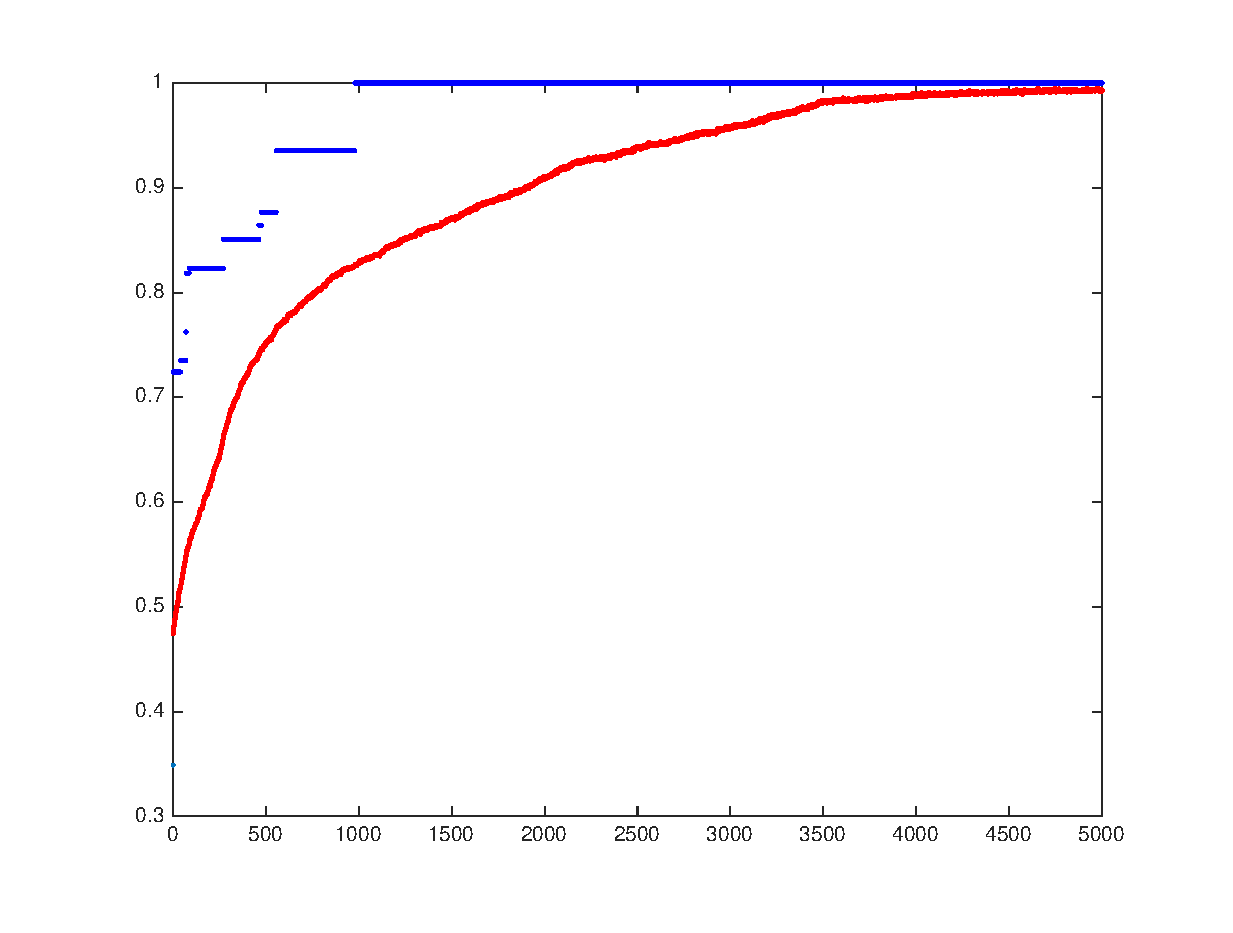
\includegraphics[width=100mm]{ER_11_200}
	\caption{test}
\end{figure}
Prueba de codigo matlab:
\begin{minted}{matlab}
case 0, % cruzamiento basado en orden
% elegidos i,j
% El elemento i esta en la posicion U2/V2(i)
%for k = 1:n 
%    U2(i) = find(U==i);
%    V2(i) = find(V==i);
%end
Y = U(i:j);
Z = V(i:j);
% tomaremos valores desde la posicion j+1
V2 = circshift(V,[0 -j]);
U2 = circshift(U,[0 -j]);
% los valores que no esten ya colocados
V2 = MY_setdiff(V2,Y);
U2 = MY_setdiff(U2,Z);
% los ponemos
Y = [V2(n-j+1:end) Y V2(1:(n-j))];
Z = [U2(n-j+1:end) Z U2(1:(n-j))];
\end{minted}
Tenemos n peticiones de uso de un laboratorio, cada uno con un tiempo de comienzo si y un tiempo de finalización ti para cada petición i. Asumimos que todos los tiempos de comienzo y final son diferentes. Dos peticiones entran en conflicto si se solapan (es decir si el tiempo de comienzo de una petición es anterior al tiempo de finalización de otra). Nuestro objetivo es seleccionar un mayor número de peticiones que no contengan solapamientos. (Por ejemplo si tenemos estas tres peticiones [0, 3], [2, 5], [4 7] entonces seleccionaremos la primera y la tercera). Diseña un algoritmo voraz que calcule la solución óptima.
\subparagraph{}
Necesitamos pensar en la acción de selección del algoritmo voraz que elaboraremos. Como la elección de una petición depende de si se solapa o no con el resto, y no queremos revisar todas cada vez, las ordenaremos por tiempo de comienzo. La última tarea la vamos a tomar siempre, ya que no condiciona al resto. Después escogeremos el resto teniendo en cuenta que no se solapen, de la que mayor tiempo de comienzo a la de menor. \\
\begin{figure}
	\centering
	\begin{subfigure}[t]{0.45\textwidth}
	\includegraphics[width=\linewidth]{../../Semestre6/COMPU/TSP/OX}
	\end{subfigure}
	\centering
	\begin{subfigure}[t]{0.45\textwidth}
	\includegraphics[width=\linewidth]{../../Semestre6/COMPU/TSP/ER11}
	\end{subfigure}
	\caption{asd}
	\label{fig:OX}
\end{figure}

\end{document}
